\documentclass[11pt]{article}

\usepackage[T1]{fontenc}
\usepackage[utf8]{inputenc}
\usepackage{lmodern}
\usepackage{amsmath,amssymb}
\usepackage{geometry}
\usepackage{hyperref}
\usepackage{graphicx}
\usepackage{float}

\geometry{margin=1in}
\graphicspath{{./}{docs/}}

% Improve spacing in align environments
\setlength{\jot}{10pt}

\title{Triplet Phase-Lock:\\
A Dual-Path Framework for Distinguishing Construction from Assignment}

\author{Dan Hawkley}
\date{}

\begin{document}

\maketitle

\begin{abstract}
Triplet phase-lock introduces a minimal framework for distinguishing constraint-preserving construction from unconstrained assignment in mathematical and computational systems. The method organizes reasoning into staged triplets and separates outcomes into two paths: invalid assignment (IA) and valid construction (VC). A classification system (ZABCD) captures failure modes, while a construction model (ABCD) defines valid systems. The examples and constructions are reproducible via Python/Jupyter notebooks (Colab-compatible) provided in the linked repository.
\end{abstract}

\section{Introduction}

Mathematical reasoning often conflates construction with assignment. Identical structures can produce different outcomes depending on whether relationships are constraint-preserving or arbitrarily assigned.

This distinction is often implicit; here it is made explicit and testable.

This work introduces a minimal framework to separate these cases:
\begin{itemize}
\item dual-path system (IA vs VC)
\item staged triplet structure
\item ZABCD failure classification
\item ABCD construction model
\item reproducible notebook implementation
\end{itemize}

\begin{figure}[t]
\centering
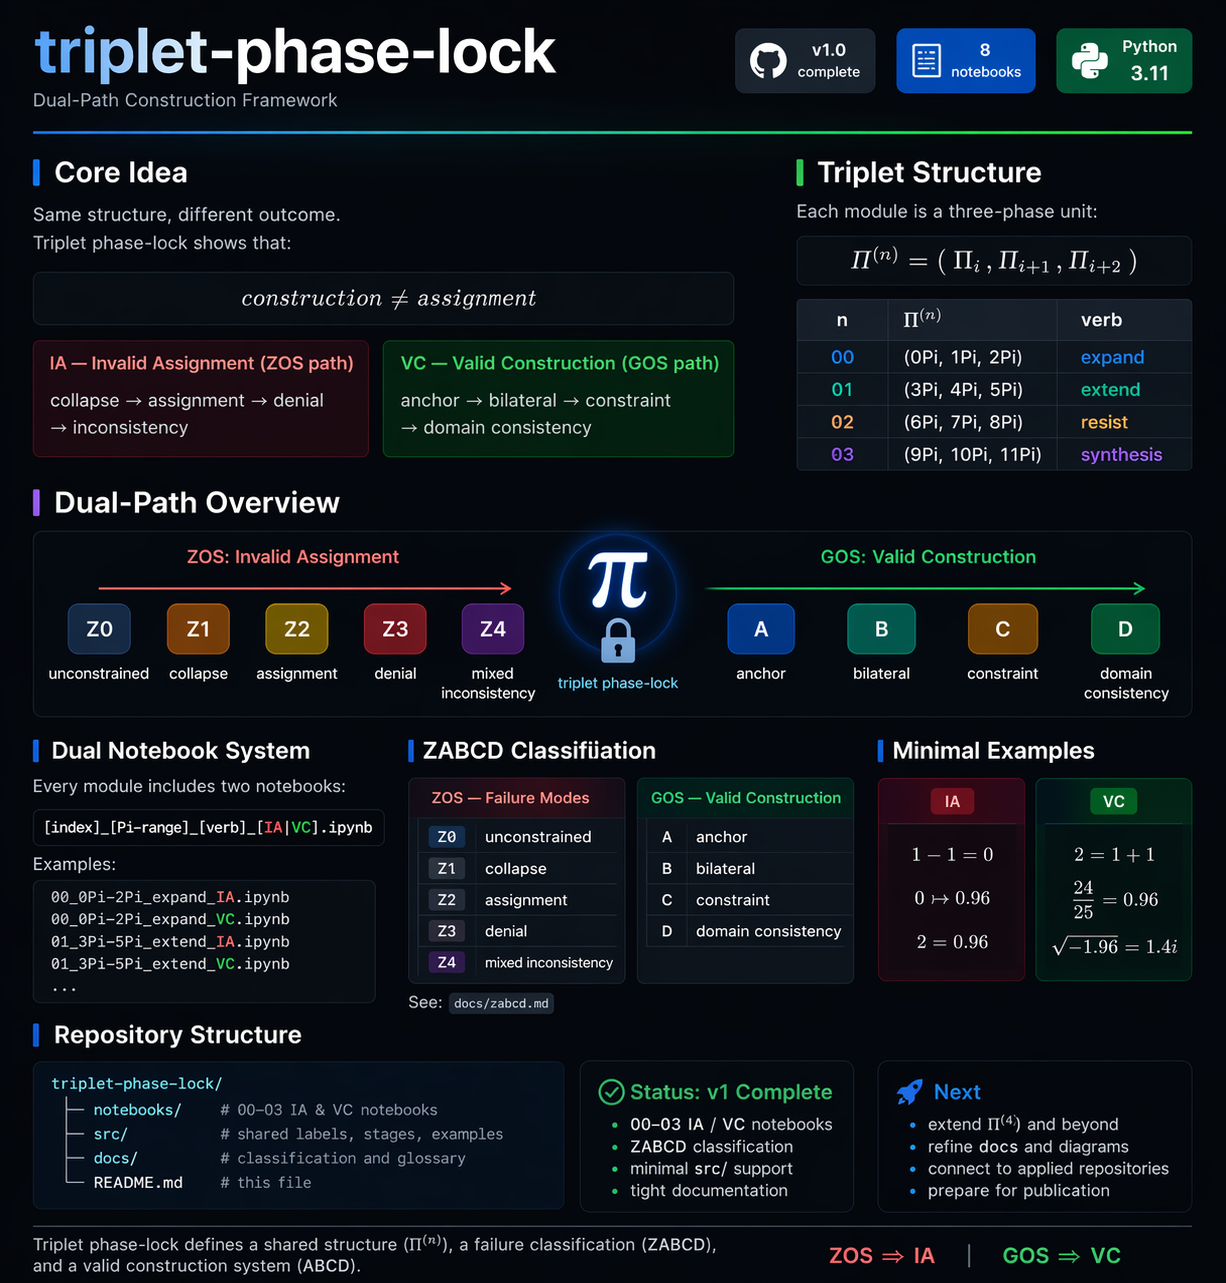
\includegraphics[width=0.88\linewidth]{banner.png}
\caption{Triplet phase-lock visual overview. The framework separates a shared staged structure into two outcomes: IA (invalid assignment, ZOS path) and VC (valid construction, GOS path).}
\label{fig:triplet-phase-lock-overview}
\end{figure}

\section{Core Definitions}

\subsection{Construction vs Assignment}

\begin{equation}
\text{construction} \neq \text{assignment}
\end{equation}

\begin{itemize}
\item Construction: constraint-preserving relations
\item Assignment: unconstrained mappings
\end{itemize}

\subsection{Dual Paths}

\begin{itemize}
\item IA: invalid assignment (ZOS path)
\item VC: valid construction (GOS path)
\end{itemize}

\subsection{Triplet Structure}

\begin{equation}
\Pi^{(n)} = (P_i, P_{i+1}, P_{i+2})
\end{equation}

Each stage shares structure while diverging in outcome.

\section{ZABCD Classification (Failure Modes)}

\begin{itemize}
\item Z0: unconstrained
\item Z1: collapse
\item Z2: assignment
\item Z3: denial
\item Z4: mixed inconsistency
\end{itemize}

Failures arise from missing structure or domain violations.

\section{ABCD Construction Model}

\begin{itemize}
\item A: anchor
\item B: bilateral
\item C: constraint
\item D: domain consistency
\end{itemize}

Valid systems satisfy all components simultaneously.

\section{Triplet Progression}

\begin{figure}[t]
\centering

\includegraphics[width=0.86\linewidth]{triplet_progression_light.png}
\caption{Triplet progression across $\Pi^{(0)}$--$\Pi^{(3)}$. IA accumulates from unconstrained states to mixed inconsistency, while VC accumulates anchor, bilateral structure, constraint, and domain consistency.}
\label{fig:triplet-progression}
\end{figure}

\subsection{$\Pi^{(0)}$ --- expand (0Pi--2Pi)}

\begin{itemize}
\item IA: Z0 $\rightarrow$ Z1 $\rightarrow$ Z2
\item VC: A $\rightarrow$ B
\end{itemize}

\subsection{$\Pi^{(1)}$ --- extend (3Pi--5Pi)}

\begin{itemize}
\item IA: Z2 $\rightarrow$ Z3
\item VC: C $\rightarrow$ D
\end{itemize}

\subsection{$\Pi^{(2)}$ --- resist (6Pi--8Pi)}

\begin{itemize}
\item IA: Z3 $\rightarrow$ Z4
\item VC: C $\rightarrow$ D
\end{itemize}

\subsection{$\Pi^{(3)}$ --- synthesis (9Pi--11Pi)}

\begin{itemize}
\item IA: Z4
\item VC: A + B + C + D
\end{itemize}

\section{Minimal Examples}

\subsection{Invalid Assignment (IA)}

\begin{align}
1 - 1 &= 0 \\[6pt]
0 &\mapsto 0.96 \\[6pt]
2 &= 0.96
\end{align}

\subsection{Valid Construction (VC)}

\begin{align}
2 &= 1 + 1 \\[6pt]
\frac{24}{25} &= 0.96 \\[6pt]
\sqrt{-1.96} &= 1.4i
\end{align}

\section{Implementation}

The framework is implemented as paired Python/Jupyter notebooks (available in the linked repository):

\begin{itemize}
\item IA path notebooks
\item VC path notebooks
\item stages 00--03 (expand, extend, resist, synthesis)
\end{itemize}

Supporting modules include:

\begin{itemize}
\item stage definitions
\item classification labels
\item minimal examples
\end{itemize}

Repository:

\begin{center}
\url{https://github.com/thinkthoughts/triplet-phase-lock}
\end{center}

\section{Interpretation}

\begin{equation}
ZOS \Rightarrow IA \qquad GOS \Rightarrow VC
\end{equation}

\begin{itemize}
\item IA accumulates inconsistency
\item VC accumulates structure
\end{itemize}

\section{Applications}

\begin{itemize}
\item debugging mathematical reasoning
\item identifying invalid mappings
\item clarifying model assumptions
\item cross-domain consistency analysis
\end{itemize}

\section{Conclusion}

Triplet phase-lock provides:

\begin{itemize}
\item a structural grammar ($\Pi^{(n)}$)
\item a classification of failure (ZABCD)
\item a model of valid construction (ABCD)
\end{itemize}

The framework is minimal, reproducible, and extensible.

\section{Future Work}

\begin{itemize}
\item extend $\Pi^{(4)}$ and beyond
\item formal validation rules
\item applications to physics and machine learning
\item integration with computational workflows
\end{itemize}

\end{document}
